\documentclass[conference]{IEEEtran}
\IEEEoverridecommandlockouts
% The preceding line is only needed to identify funding in the first footnote. If that is unneeded, please comment it out.
\usepackage{cite}
\usepackage{amsmath,amssymb,amsfonts}
\usepackage{algorithmic}
\usepackage{graphicx}
\usepackage{textcomp}
\usepackage{xcolor}
\usepackage{multirow}
\usepackage{balance}
\def\BibTeX{{\rm B\kern-.05em{\sc i\kern-.025em b}\kern-.08em
    T\kern-.1667em\lower.7ex\hbox{E}\kern-.125emX}}
\begin{document}

\title{Handling out of vocabulary words at the semantical level using recurrent neural networks\\\vspace{0.75cm}
\thanks{Funding information suppressed due to blind-review.}
}

\author{\IEEEauthorblockN{Paula Pedroso}
\IEEEauthorblockA{\textit{Technological Sciences Center} \\
\textit{State University of Maranhão}\\
São Luís, Brazil \\
paulapedroso@aluno.uema.br}
\and
\IEEEauthorblockN{Antonio Jacob}
\IEEEauthorblockA{\textit{Technological Sciences Center} \\
\textit{State University of Maranhão}\\
São Luís, Brazil \\
antoniojunior@professor.uema.br}
\and
\IEEEauthorblockN{Fábio Lobato }
\IEEEauthorblockA{\textit{Engineering and Geosciences Institute} \\
\textit{Federal University of Western Pará}\\
Santarém, Brazil \\
fabio.lobato@ufopa.edu.br}
\and
{\IEEEauthorblockN{Eveline Sá }
\IEEEauthorblockA{\textit{Computer Department} \\
\textit{Federal Institute of Maranhão}\\
São Luís, Brazil \\
eveline@ifma.edu.br}
}
}

\maketitle

\begin{abstract}

Text recognition through natural language processing (NLP) faces challenges when it encounters a word that is not categorized. These types of words are called out-of-vocabulary words (OOV). They are often the subject of representation, local slang, or typing mistakes. These types of content have grown exponentially as the Internet has popularized, making people interact more assiduously through texting. Given the importance of this subject, we present three OOV classification models based on deep learning using a corpus with words in Portuguese as a case study. These models are bidirectional simple recurrent neural networks (RNN), short-term long memory (LSTM), and gated recurrent units (GRU). The purpose is to enable the system to recognize the embedding of OOV and place them in a vector space. In addition, the meaning of the words was verified using cosine similarity. The results of LSTM are promising for identifying OOV and generating semantically similar words. The model can be used in pre-processing pipelines for user-generated content analysis, adding more value to social media studies.
\end{abstract}

\begin{IEEEkeywords}
recurrent neural networks, out-of-vocabulary, natural language processing, cosine similarity
\end{IEEEkeywords}

\section{Introduction}
Natural Language Processing (NLP) is a computing area  with a range of computational techniques that aims to analyze and represent texts to achieve human-like language processing for various tasks, or applications \cite{b1}. It is widely used by researchers who seek to use words from a computational perspective \cite{b2}. The field involving the treatment of words is vast, ranging from the automatic translation to recognition of meanings and sentiment analysis \cite{b1,b23}.

In extensive research on NLP, most tasks are based on word-level methods because it is the smallest linguistic unit in natural languages \cite{b23,b26}. As treatments are the basis of words, it is inevitable that unknown words, called Out-Of-Vocabulary words (OOV), will inevitably occur. As much as it is a field in constant growth, the non-treatment of OOVs has a deleterious effect on the reliability of the analyses because it causes a loss of information in the calculations and, consequently, in decision-making \cite{b4}.

In light of this, many techniques for dealing with these types of words exist. However, some limitations are perceived, such as the non-treatment of OOVs considered variants of other OOVs or even that they are OOVs composed of typos \cite{b16}. This is evidenced when using a textual training domain that is different from NLP tasks \cite{b15}. Studies have proven that Recurrent Neural Networks (RNN) are being widely used in NLP, driven by the fact that they are characterized by having a memory of their previous states, allowing them to model sequences very well; thus, improving performance in language modeling tasks \cite{b4,b5,b26}. Considering the state-of-the-art, the following research questions (RQ) were raised:
\begin{enumerate}
     \item How to handle out-of-vocabulary words in natural language processing?
     \item Can deep learning be used to treat OOV at the semantic level?
\end{enumerate}

To answer these research questions, we employed simple RNNs, Long Short-Term Memory (LSTM), and Gated Recurrent Units (GRU) for modeling the OOV problem, using a training corpus with Portuguese words obtained from users' comments from a journalistic platform . Training consists of extracting the unknown word embedding through the context in which it is present. Through this training, the final vectors were produced and added to the vocabulary model \cite{b7}. In addition, a qualitative analysis is performed using the cosine similarity metric, which shows how two words are related based on the cosine value between the vectors \cite{b8,b9}.

This work contributes to the body of knowledge by evaluating the aforementioned methods for detecting and treating OOV. The results of LSTM are promising for identifying OOV and generating semantically similar words. The model can be used in pre-processing pipelines for User-Generated Content (UGC) analysis, adding more value to social media studies \cite{b21}. It is important to point out that regionalism and similar linguistic phenomena bring up powerful meaning to the message, which is quite common in UGC. Developing strategies for treating this issue has many industrial applications. For example, it can improve the accuracy and reliability of social customer relationship management (Social CRM) platforms \cite{b22,b21}. Moreover, the proposed approach is scalable and can be adopted in other languages.

The remainder of this paper is organized as follows. In Section 2, previous works carried out on the treatment of OOVs are discussed. Section 3 describes the materials and methods used in the experiments. In Section 4, experimental results are presented and discussed. The conclusions, suggestions for future work, and research limitations are presented in Section 5.

\section{Related Works}
Word embeddings are developed by training vector representations of words in a large text corpus. The final vectors produced were dense representations of the respective words, and the words were added to the vocabulary model \cite{b7}. Algorithms that can model embeddings more effectively are those based on neural networks, such as RNN, GRU, and LSTM \cite{b6}. These algorithms are used because they facilitate the incorporation of OOV words by exploring contextual/semantical information to extract the desired information \cite{b14}.

Similarly, Premjith, Soman, and Prabaharan \cite{b6} uses RNN, GRU, LSTM, and their bidirectional versions to generate part of speech marking for the Sanskrit language. Combinations of hyperparameters were used to achieve an accuracy score of 95.92\% with the training GRU.

Kandi \cite{b7} proposed a bidirectional LSTM model that recognizes word embedding based on its context. The objective is to efficiently predict vectors for OOV words in real-time to use them in ChatBot applications. For this, the treatment was carried out in a database in English and trained using bidirectional LSTM with hyperparameter optimization. The model input consisted of sentences, and the output was the OOV recognized and its context.

Regarding word embedding assessment, most studies use the intrinsic method that evaluates models by examining their effectiveness in providing syntactic and semantic representations of words \cite{b17}. The most common specific tasks for this type of assessment include word matching/similarity and analogy matching \cite{b17}.

Tang et al. \cite{b13} trained a database in English and used a quality assessment method to create embeddings using word similarity. This quality assessment was performed using Spearman's rank correlation to measure the relationship between two variables: the similarity score given by the neural language model and the human annotations.

Won and Lee \cite{b14} pre-trained a corpus with English words, showing the performance of the model using loss and accuracy metrics. The proposed model achieved an accuracy of 89.65\% and a loss of 0.30. For this purpose, an OOV word incorporation method is proposed that explores both the words and contextual information to extract the desired information.

As in human language, new words are often introspected, retrieving our memory to understand their meaning based on similar words or giving the new word approximate characteristics through its context \cite{b20}. In NLP terms, similar words are analogous to training samples and the context is that of the test dataset \cite{b20}.

Based on these works, we propose training recurrent neural networks with a Portuguese corpus to identify and handle OOV. This training used a combination of hyperparameters to verify the performance of the model using loss and accuracy metrics. Subsequently, a quality evaluation analysis was conducted to create embeddings based on the similarity of words. This study contributes to NLP research on the treatment of OOVs in Portuguese. The strategy adopted is scalable and can be adapted to other languages.


\section{Materials and Methods}

This section briefly describes the OOV problem and the neural models currently used to solve this issue using semantic information. The datasets used in the experiments were also defined. Finally, the proposed solution is framed in this state of the art, highlighting its objectives and contributions to research.


\subsection{Problem description}
Out-of-vocabulary words appear in the test text data, but not in the recognition vocabulary on which the text data are trained \cite{b7}. This is one of the main challenges for NLP \cite{b10}. Studies such as Kandi \cite{b7} and Tang et. al. \cite{b13}, and Won and Lee \cite{b14} sought to recognize embeddings for OOVs. \cite{b7} uses bidirectional long short-term memory to predict the most likely word to substitute the OOV word based on its context.

Tang et. al. \cite{b13} used context-sensitive long short-term memory to recognize embeddings through syntactic and semantic information in grouping-related words. Lee \cite{b14} used a contextual morphosyntactic method to extract information from OOVs and improved the quality of text classification using unseen words.

Our approach aims to identify OOV and provide candidate words in the embedding space for substituting OOVs. Based on the state-of-the-art discussed in the Related Work section, recurrent neural models are the most suitable for this task. In the following subsection, we present the methods used in our experiments.


\subsection{Algorithms for handling OOV}
The algorithm that models this problem must remember the context effectively to identify the label, and algorithms based on recurrent neural networks are capable of storing context dependencies. Therefore, it is used to predict the labels of the entities in a given sequence \cite{b6}.

\subsubsection{Simple Recurrent Neural Networks}
They are designed to work with sequential data and can be time series in text, audio, image, or video formats. They use previous information in the sequence to produce the current output and have short-term memory \cite{b6}. It is a deep learning model applied to process data in a sequential order such that the input of a particular state depends on the output of the previous state \cite{b18}. The basic architecture of an RNN is illustrated in Figure \ref{fig4}.

\begin{figure}[htbp]
\centerline{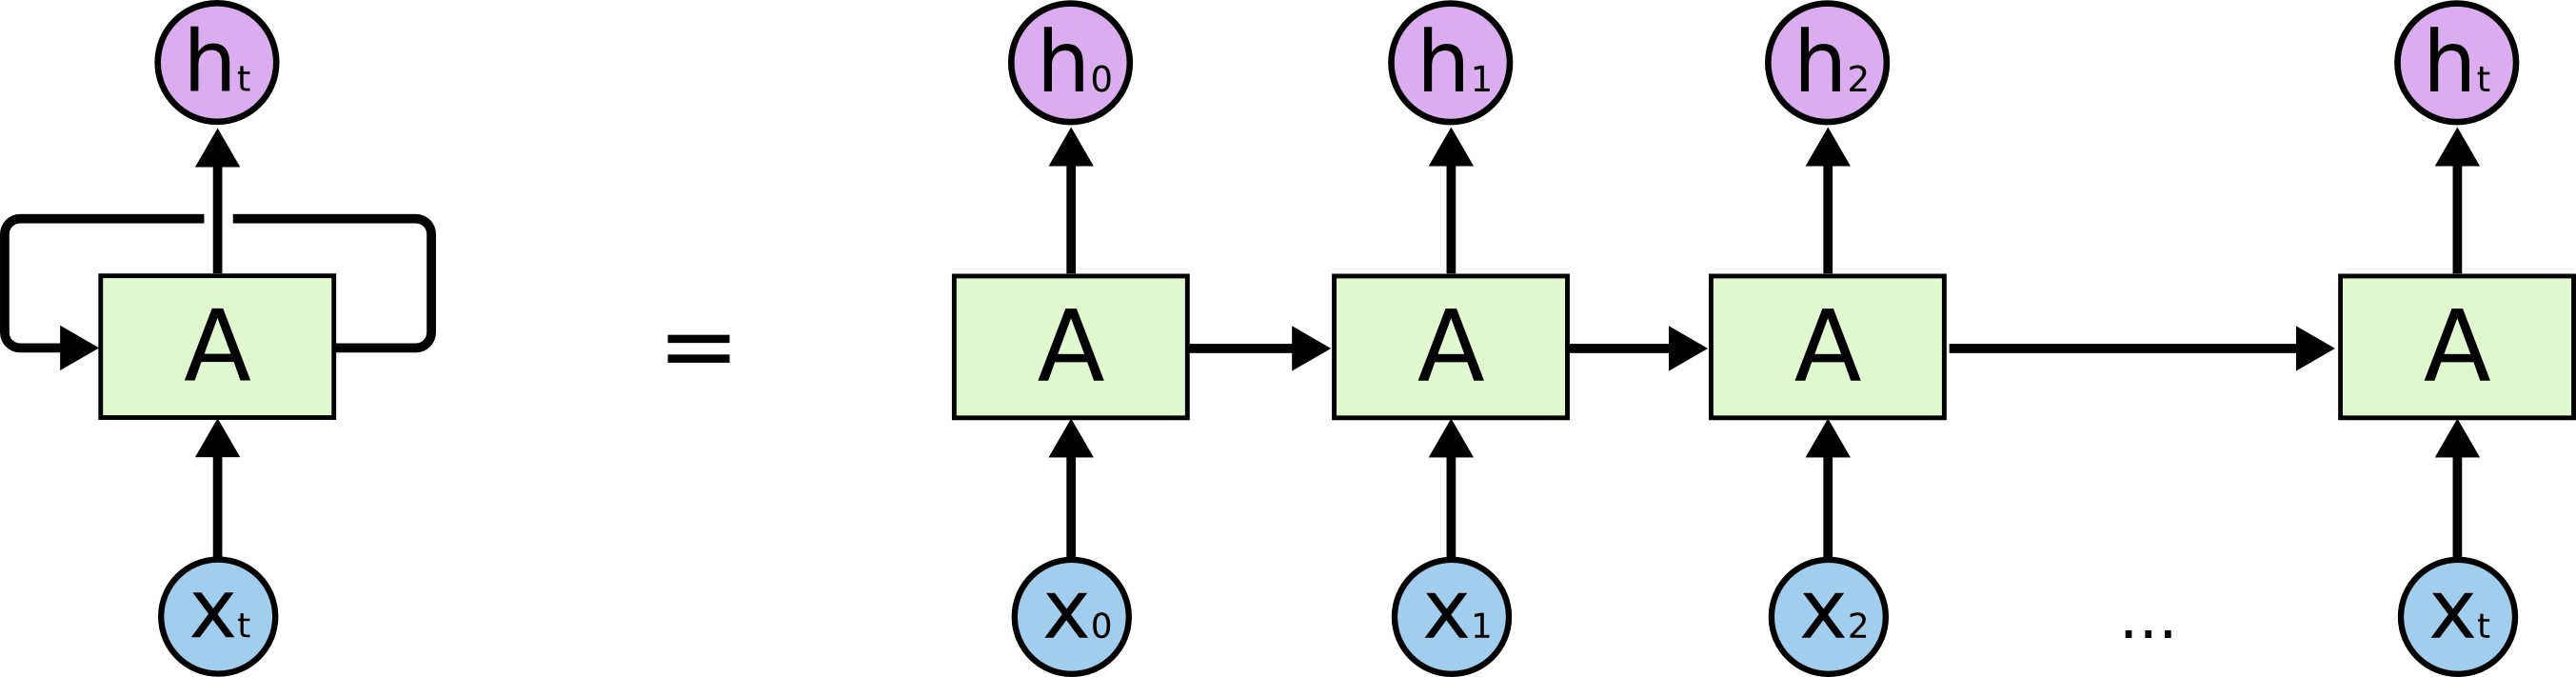
\includegraphics[scale=0.2]{images/rnn.png}}
\caption{Canonical architecture of an RNN.}
\label{fig4}
\end{figure}

Figure \ref{fig4} shows the unfolding of an RNN, which means that the network is split into complete sequences. For example, if a sequence contains a sentence with five words, the network would be unfolded into a 5-layer neural network, that is, one layer for each word.

This recurring model includes a hidden state that determines the previous rank in a series, and at each subsequent step, this hidden state is combined with the input data from the new step to produce a new hidden state \cite{b18}. It then reclassifies, causing this hidden state to be recycled to produce a modified successor. Practically, an RNN can only keep track of the immediate past, and it suffers from the problem of vanishing/exploding gradients when dealing with long-range contextual dependencies
\cite{b6}.

\subsubsection{Long Short-Term Memory}
LSTM is an architecture that aims to solve the vanishing gradient problem. LSTM is a neural network capable of learning order dependence in sequence-prediction problems. This is an RNN architecture with long-term memory \cite{b13}. An LSTM network can remember the context for a long time with the help of some specially designed gate circuits \cite{b6}. LSTM works similarly to RNN in terms of unfolding, but LSTM has a chain structure that contains different memory blocks called cells. The basic architecture of an LSTM cell is illustrated in Figure \ref{fig5}.

\begin{figure}[htbp]
\centerline{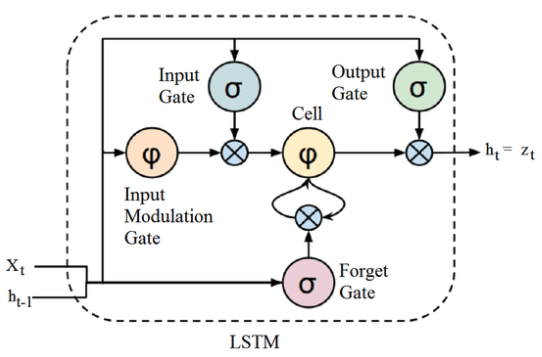
\includegraphics[scale=0.4]{images/lstm.png}}
\caption{Basic cell architecture of the LSTM network.}
\label{fig5}
\end{figure}

The Figure shows the following gates, as defined in \cite{b6}:
\begin{enumerate}
    \item \textbf{Input Modulation Gate:} Cells retain information, and gates do memory manipulations;
    \item \textbf{Forget Gate:} Information that is no longer useful in cell state is removed;
    \item \textbf{Input gate:} This gate adds useful information to the cell state;
    \item \textbf{Output gate:} The task of extracting useful information from the state of the current cell is to be presented as output;
    \item \textbf{Cell:} The looped arrows in Figure \ref{fig5} indicate the recursive nature of the cell, causing information from previous ranges to be stored in the LSTM cell.


\end{enumerate}




\subsubsection{Gated Recurrent Units}
It is the most recent generation of RNN and is quite similar to LSTM. It can be used to improve the memory capacity of a neural network and provide the facility to train a model, as it decides whether such information should be updated within a cell \cite{b6}. This architecture has only two gates, a reset gate, and an update gate, as shown in Figure \ref{fig6}.

\begin{figure}[htbp]
\centerline{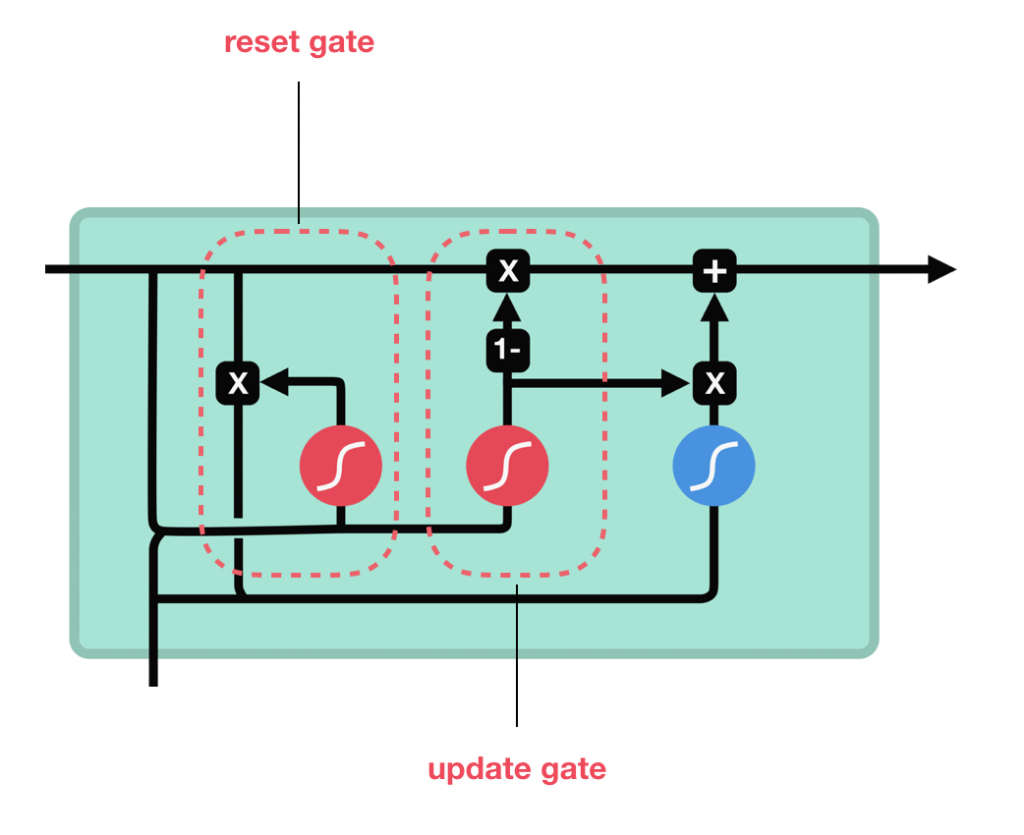
\includegraphics[scale=0.2]{images/gru.png}}
\caption{Canonical architecture of the GRU.}
\label{fig6}
\end{figure}

Figure \ref{fig6} shows the following gates according to \cite{b6}:
\begin{enumerate}
    \item \textbf{Reset gate:} This decides how to merge the time-step input with the time-step contextual information;
    \item \textbf{Update gate:} This gate is used to calculate the amount of past information to be stored in the current state.
\end{enumerate}

They are two vectors that determine the information to pass to the output. They can be trained to retain old information without dissipating it over time or removing information irrelevant to the forecast.


\subsection{Dataset Description}
The corpus\footnote[1]{https://github.com/fabiolobato/OOV-WebIntelligence2022} is composed of an extract of Portuguese news from the Portal G1 website. Alexa\footnote[2]{https://www.alexa.com/topsites/countries/BR} ranking was based on the ability to use the G1 website, as was also used in the work of Rodrigues et al. \cite{b11} and \cite{b28}. Basic information regarding the news was collected, such as the title, abstract, complete news, publication date, and access link. For this purpose, the algorithm proposed by Rodrigues et al. \cite{b11} was delimited to the following search terms:
\begin{itemize}
\item \textit{Pão com ovo}
\item \textit{Bumba-boi}
\item \textit{Muleque té doido}
\item \textit{Ludovisence}
\end{itemize}
These search terms were chosen to find words from the Maranhão vocabulary in order to have many words unknown by traditional models. After the extraction, treatment of the corpus was carried out to leave only the complete news and extraction of \textit{links} in the base, as performed by Sousa et al. \cite{b24}. As the text did not have \textit{emojis} (images that convey word ideas), it was not necessary to perform other types of pre-processing, such as Rodrigues et al. \cite{b11}, by removing \textit{stopwords}, punctuation, special characters, \textit{emojis}, greetings, and accents. This method of making a database noisy was proposed by Jettakul et al. \cite{b15} to observe the effect of this type of database on the performance of the models.

\subsection{Word similarity}
The cosine similarity is a measure that evaluates the cosine value of the angle between two vectors to determine the similarity between them \cite{b9}. It is used to calculate the similarity of contextual words, where OOV morphological variants and missing words are processed by the algorithm \cite{b8}.

The cosine similarity between the word vectors
\begin{math} 
A = \{a_1, a_2,\ldots,a_n\}
\end{math}
and 
\begin{math} 
B = \{b_1,b_2,\ldots,b_n\} 
\end{math}
is calculated using Equation \ref{cosine}.
\begin{equation}
\label{cosine}
cos(\pmb A, \pmb B) = \frac {\pmb A \cdot \pmb B}{||\pmb A|| \cdot ||\pmb B||}
\end{equation}

The cosine distance between two words (or the corpus) is calculated using the dot product of two numeric vectors. It is normalized by the product of the vector lengths such that output values close to 1 indicate high similarity \cite{b8}. A high similarity means that the vectors are oriented in the same direction, and the angle is close to 0°; therefore, the cosine of the angle is close to 1 \cite{b7}.


\section{Experiments and Results}

To generate embeddings of words outside the vocabulary, three language models were used using recurrent neural networks with their unidirectional versions: RNN, LSTM, and GRU. According to Yang et al. \cite{b20}, it is necessary to train the models to handle OOVs. These models predict vectors for OOV words using the sentences in which they are projected through the context. The database used in this research had 18,997 words, 160,880 sequences, and a maximum sequence length of 2,010, as shown in Table \ref{tab1}.

\begin{table}[htbp]
\caption{Corpus Information}
\begin{center}
\begin{tabular}{|ll|}
\hline
\multicolumn{1}{|l|}{\textbf{Aspect}}     & \textbf{Value} \\ \hline
\multicolumn{1}{|l|}{Vocabulary Size}     & 18,997 \\ \hline
\multicolumn{1}{|l|}{Total Sequences}     & 159,420 \\ \hline
\multicolumn{1}{|l|}{Max Sequence Length} & 2,010   \\ \hline
\end{tabular}
\label{tab1}
\end{center}
\end{table}

The corpus used in this work is relatively smaller than that used in the works of Won and Lee \cite{b14} (vocabulary size greater than 120,000) and Soman and Prabaharan \cite{b6} (Vocabulary Size 34,270).

Initially, a tokenization process is performed, which is used to adjust the source text to represent each word using a vector. These vectors, represented by integers, can be used to sequence the text lines. These sequences are then split into input and output elements for use in the RNN, LSTM, and GRU prediction models. This process was performed three times for testing purposes between models using the same corpus and sequencing data.

The training organization was proposed by Gulli and Pal \cite{b19}, where the model is defined as sequential, an embedding layer is created, the input and output dimensions are specified, and a forecast model layer is added. This step is different for each forecast model because it is separated by architecture, as shown in Figure \ref{fig1}.

\begin{figure*}[!ht]
\centerline{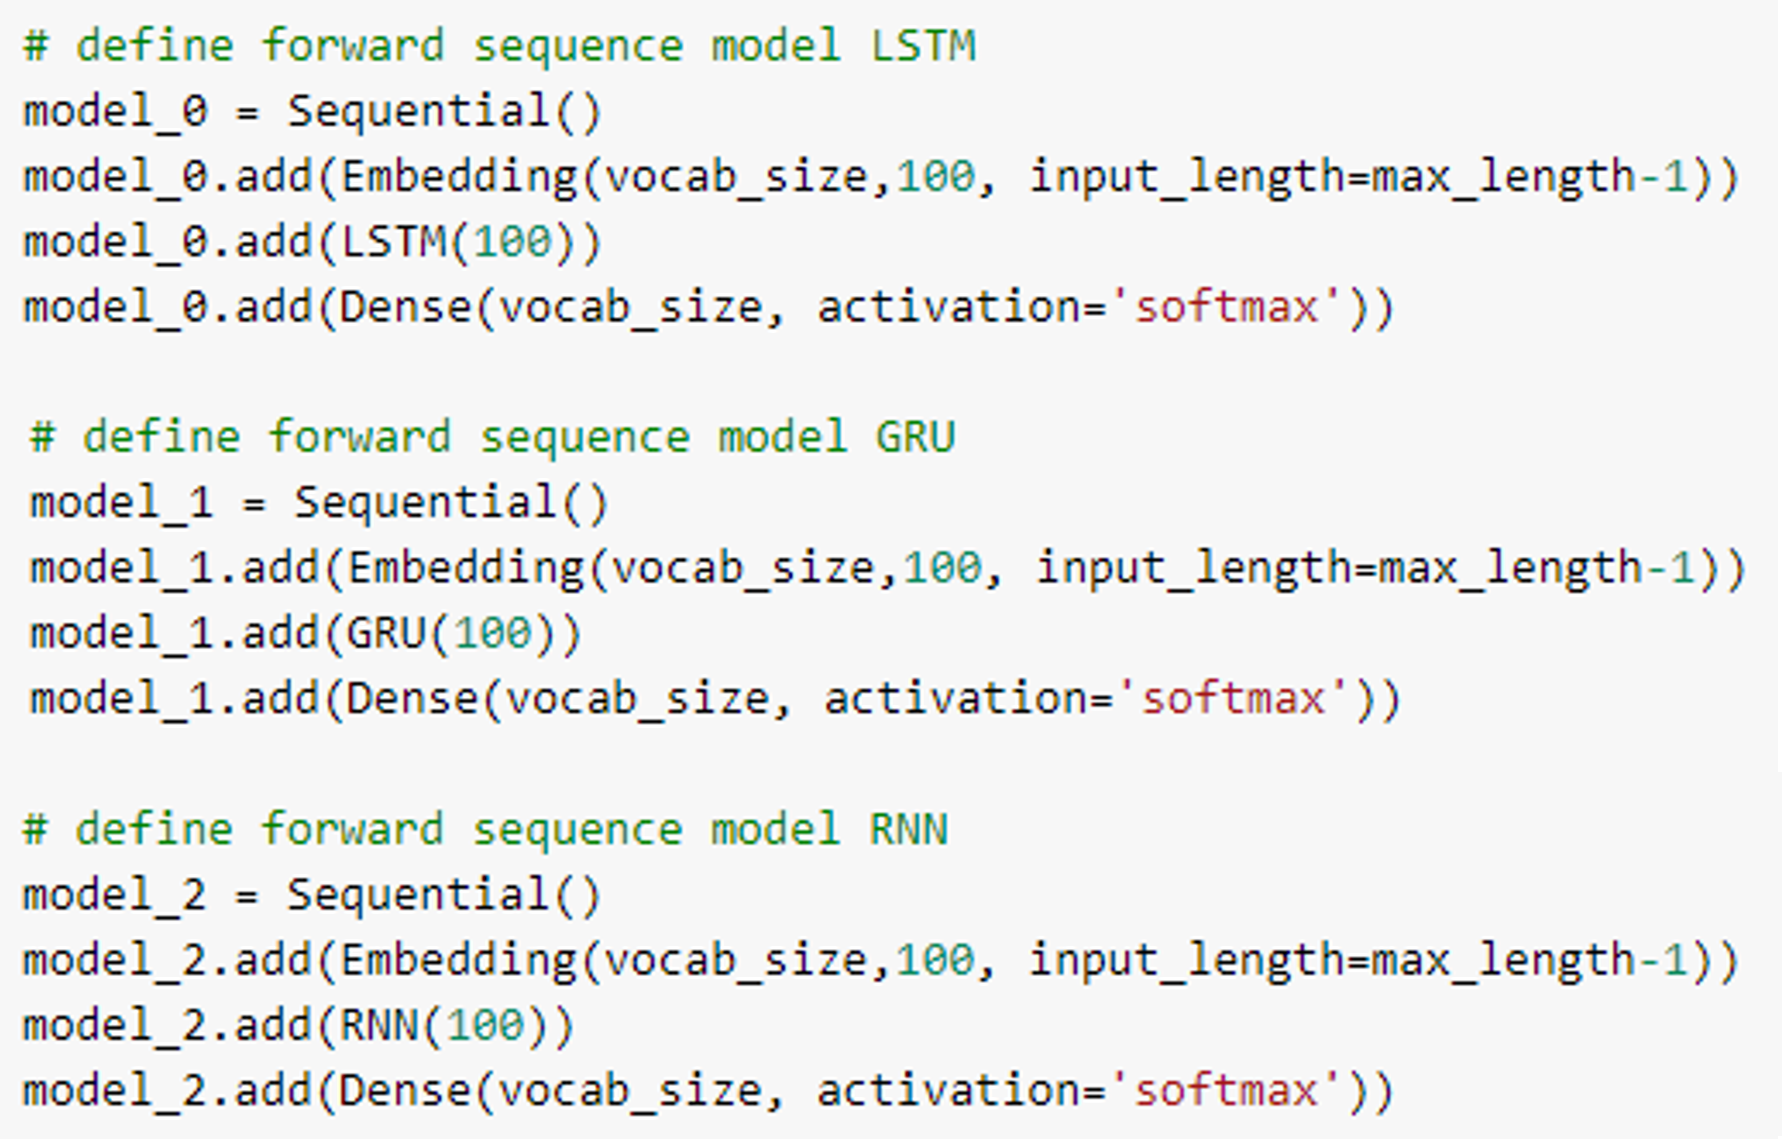
\includegraphics[scale=1]{images/Picture1.png}}
\caption{Snippet that defines prediction models.}
\label{fig1}
\end{figure*}

Figure \ref{fig1} also shows that the output layer has been defined as a dense layer composed of the vocabulary size together with a SoftMax function, as it helps ensure that the output is normalized to return a probability \cite{b7,b10,b12}. After defining the model, it was compiled and trained using the hyperparameters listed in Table \ref{tab2}.

\begin{table}[htbp]
\caption{Hyperparameters and their values used for this work}
\begin{center}
\begin{tabular}{|l|l|}
\hline
\textbf{Hyperparameters} & \textbf{Parameter value} \\ \hline
Number of epochs         & 200                      \\ \hline
Batch size               & 100                      \\ \hline
Verbose                  & 2                        \\ \hline
Learning rate            & 0.01                     \\ \hline
Optimizer                & Adam                     \\ \hline
Embedding size           & 100                      \\ \hline
\end{tabular}
\label{tab2}
\end{center}
\end{table}

Table \ref{tab2} shows that the learning rate was set to 0.01 with the Adam optimizer, and the number of epochs was set to 200 with a batch size of 100. Verbose was set to 2 because one row had to be defined for each training with information on accuracy and loss \cite{b19} to generate information for assembling the graphs of Figures \ref{fig2} and \ref{fig3}. An embedding size of 100 and the other hyperparameters were obtained following Kandi’s recommendation \cite{b7}, as the algorithm model built in the Jupyter Notebook environment using Python 3 programming language was used, the same used in his work. After training the models, it was possible to obtain the progress of accuracy and loss of each, as shown in Figures \ref{fig2} and \ref{fig3}, respectively.

\begin{figure}[htbp]
\centerline{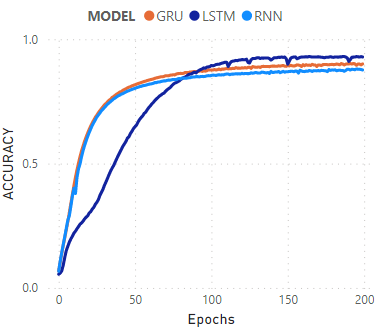
\includegraphics[scale=0.75]{images/acc.PNG}}
\caption{Accuracy training curve.}
\label{fig2}
\end{figure}

Figure \ref{fig2} shows that as the training epochs pass, the accuracy percentage of the models increases, and the three models started with very similar accuracy measures. It is also clear that the RNN and GRU models are the closest in terms of accuracy percentages throughout training and were also the ones that reached higher peaks of accuracy in a shorter training interval, with the increase being reduced after 50 training epochs. The LSTM model increased its accuracy more slowly, reaching 200 epochs with a higher percentage than the other models.

\begin{figure}[htbp]
\centerline{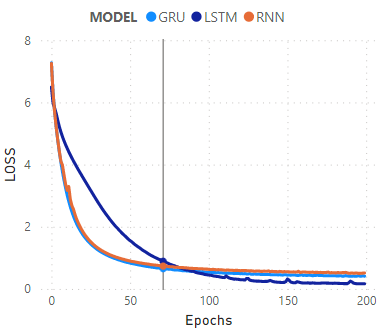
\includegraphics[scale=0.75]{images/loss.PNG}}
\caption{Loss training curve.}
\label{fig3}
\end{figure}

Figure \ref{fig3} shows that as the training epochs pass, the loss value of the models' decreases. The RNN and GRU models achieved higher peaks of loss reduction in a shorter training interval, and the LSTM decreased more slowly, as was the case with the accuracy measurement.

The choice of hyperparameters helped achieve a good convergence in the learning curve, as shown in Figures \ref{fig2} and \ref{fig3}, given the corpus used for training.

As described by Yang et al. \cite{b20}, accuracy is used to measure the performance of the algorithm, and the loss value indicates how poorly or well a model behaves after each optimization iteration. Therefore, the higher the accuracy, the better the algorithm, and the lower the loss, the better the performance of the model.

In the analysis, it was possible to verify that the LSTM model was the one that obtained the best performance (higher accuracy and lower loss). At the end of training, absolute values were generated, as shown in Table \ref{tab3}.

\begin{table}[!ht]
\caption{Results summarization for the models considered in the experiments.}
\begin{center}
\begin{tabular}{|l|l|l|l|}
\hline
\textbf{\begin{tabular}[c]{@{}l@{}}Classification \\ Algorithm\end{tabular}} & \textbf{Accuracy} & \textbf{Loss} & \textbf{\begin{tabular}[c]{@{}l@{}}Training \\ time \end{tabular}} \\ \hline
RNN  & 87.66\% & 0.5141  & 4 days  \\ \hline
LSTM & \textbf{93.32\%} & \textbf{0.2785}  & 10 days \\ \hline
GRU  & 90.06\% & 0.4113  & 8 days  \\ \hline
\end{tabular}
\label{tab3}
\end{center}
\end{table}

The values presented in Table \ref{tab3} confirm that LSTM outperformed the other methods, as it achieved an accuracy of 93.32\% and a loss of 0.2785. However, 10 days were required for the training. We found that this result was better than that reported by Won and Lee \cite{b14} (89.65\%) but lower than that reported by Premjith, Soman, and Prabaharan \cite{b6} (95.92\%). In this scenario, it is worth highlighting the study by Kim et al. \cite{b16}, which proved that databases with different languages have different behaviors in the training results despite having the same parameters.

After training the models, quality verification was performed using the cosine similarity function. As in Won et al. \cite{b9}, tests were carried out with random sentences containing unknown words and a similarity check with sentences with the exact content of context. The results are presented in Table \ref{tab4}.

\begin{table*}[htbp] \footnotesize
\caption{Sentence similarity test result}
\begin{center}
\begin{tabular}{|l|l|lll|}
\hline
\multicolumn{1}{|c|}{\multirow{2}{*}{\textbf{Sentence with OOV}}}                                                                            & \multicolumn{1}{c|}{\multirow{2}{*}{\textbf{Test sentence}}}                                                                                                               & \multicolumn{3}{c|}{\textbf{Model}}                                                     \\ \cline{3-5} 
\multicolumn{1}{|c|}{}                                                                                                                       & \multicolumn{1}{c|}{}                                                                                                                                                      & \multicolumn{1}{l|}{\textbf{GRU}}  & \multicolumn{1}{l|}{\textbf{LSTM}} & \textbf{RNN}  \\ \hline
Tua atitude foi muito \textbf{bandeirosa} durante a festa.                                                                                            & As pessoas por aqui são muito \textbf{indiscretas}.                                                                                                                                 & \multicolumn{1}{l|}{\textbf{0.06}} & \multicolumn{1}{l|}{0.05}          & 0.00          \\ \hline
\begin{tabular}[c]{@{}l@{}}Não é utilizado nenhum título \textbf{bandeiroso}, mas ao invés \\ disso, damos ênfase à veracidade dos fatos\end{tabular} & \begin{tabular}[c]{@{}l@{}}Dario já viu fotos de sadomasoquismo, mas nada tão \\ \textbf{escandaloso} que não pudesse ser encontrado na banca \\ de jornais da esquina\end{tabular} & \multicolumn{1}{l|}{0.56}          & \multicolumn{1}{l|}{\textbf{0.65}} & 0.37          \\ \hline
O problema de sair com ele é que ele é muito \textbf{bandeiroso}.                                                                                     & \begin{tabular}[c]{@{}l@{}}Você não pode ser tão \textbf{descuidado}, tudo o que pega na mão\\ você deixa cair\end{tabular}                                                         & \multicolumn{1}{l|}{0.51}          & \multicolumn{1}{l|}{\textbf{0.72}} & 0.39          \\ \hline
\textbf{Mermã}, e o quê que aconteceu ontem?                                                                                                          & você é minha melhor \textbf{amiga}.                                                                                                                                                 & \multicolumn{1}{l|}{\textbf{0.35}} & \multicolumn{1}{l|}{\textbf{0.35}} & \textbf{0.35} \\ \hline
Eu te avisei sobre isso, \textbf{mermã}.                                                                                                              & Não faça mais isso minha \textbf{colega}                                                                                                                                            & \multicolumn{1}{l|}{0.25}          & \multicolumn{1}{l|}{0.27}          & \textbf{0.36} \\ \hline
ei \textbf{mermã}, vamos sair hoje?!                                                                                                                  & Onde está a minha \textbf{irmã}?                                                                                                                                                    & \multicolumn{1}{l|}{0.07}          & \multicolumn{1}{l|}{0.32}          & \textbf{0.41} \\ \hline
\begin{tabular}[c]{@{}l@{}}Ana Maria contratou um sanfoneiro \textbf{paidégua} para tocar\\ no aniversário do marido.\end{tabular}                    & Camões foi um homem \textbf{valoroso}.                                                                                                                                              & \multicolumn{1}{l|}{0.25}          & \multicolumn{1}{l|}{0.15}          & \textbf{0.45} \\ \hline
Essa festa tá \textbf{paidégua}.                                                                                                                      & É muito \textbf{legal} brincar no computador.                                                                                                                                       & \multicolumn{1}{l|}{0.08}          & \multicolumn{1}{l|}{-0.01}         & \textbf{0.34} \\ \hline
Aquele suco de acerola é \textbf{paidégua}                                                                                                            & Este lanche está \textbf{gostoso}.                                                                                                                                                  & \multicolumn{1}{l|}{0.10}          & \multicolumn{1}{l|}{0.01}          & \textbf{0.31} \\ \hline
Aquela sua ex-namorada tava \textbf{marocando} meu facebook                                                                                           & \begin{tabular}[c]{@{}l@{}}Também foi possível \textbf{observar} que os freios sobre as asas \\ permaneceram levantados\end{tabular}                                                & \multicolumn{1}{l|}{-0.15}         & \multicolumn{1}{l|}{\textbf{0.43}} & 0.38          \\ \hline
A vizinha estava \textbf{marocando} a minha vida.                                                                                                     & Elas ficam \textbf{fofocando} no meio da praça                                                                                                                                      & \multicolumn{1}{l|}{0.12}          & \multicolumn{1}{l|}{0.17}          & \textbf{0.19} \\ \hline
Vou entrar no instagram pra \textbf{marocar}.                                                                                                         & \begin{tabular}[c]{@{}l@{}}A instituição informou que continuará \textbf{vigiando} a atividade \\ do vulcão\end{tabular}                                                            & \multicolumn{1}{l|}{-0.03}         & \multicolumn{1}{l|}{\textbf{0.40}} & -0.08         \\ \hline
\end{tabular}
\label{tab4}
\end{center}
\end{table*}

According to the similarity results, it can be seen that the RNN and LSTM models obtained similar scores, namely for the words ``Bandeiroso \ Bandeirosa'' and ``Marocar'' the LSTM was better and for the words ``Mermã'' and ``Paidégua'' the RNN was the winner. The bold values in Table \ref{tab4} indicate the best results.

It was used for test words with different grammatical classes. For this, we verified the grammatical marking of each word together with its real meaning, obtained from the dictionary proposed by Neres and Barros \cite{b25}, as shown in Table \ref{tab_bis}.

\begin{table}[!ht]
\caption{Word meaning.}
\begin{center}
\begin{tabular}{|l|l|l|}
\hline
\multicolumn{1}{|c|}{\textbf{Word}}                              & \multicolumn{1}{c|}{\textbf{Meaning}}                                           & \multicolumn{1}{c|}{\textbf{\begin{tabular}[c]{@{}c@{}}Part-of-Speech\\ tagging\end{tabular}}} \\ \hline
\begin{tabular}[c]{@{}l@{}}Bandeiroso,\\ Bandeirosa\end{tabular} & \begin{tabular}[c]{@{}l@{}}Escandaloso,\\ Indiscreto,\\ Descuidado\end{tabular} & adjective                                                                                      \\ \hline
Mermã                                                            & \begin{tabular}[c]{@{}l@{}}Amiga,\\ Irmã,\\ Colega\end{tabular}                 & substantive                                                                                    \\ \hline
Paidégua                                                         & \begin{tabular}[c]{@{}l@{}}Bom, Valoroso,\\ Legal\end{tabular}                  & adjective                                                                                      \\ \hline
Marocar                                                          & \begin{tabular}[c]{@{}l@{}}Fofocar,\\ Observar,\\ Vigiar\end{tabular}           & verb                                                                                           \\ \hline
\end{tabular}
\label{tab_bis}
\end{center}
\end{table}

The Table \ref{tab_bis} shows the meanings of the words ``Bandeiroso / Bandeirosa,'' ``Mermã,'' ``Paidégua'' and ``Marocar,'' according to research by Neres and Barros \cite{b25}. These meanings were based on the vocabulary of the state of Maranhão. Through these meanings, sentences that contained the same context to be assigned in the similarity tests were defined.

\section{Conclusions}
There are several open problems in the NLP field, in which out-of-vocabulary words deserve attention. Correct handling OOV has the potential to be included in the pre-processing pipeline to improve analysis reliability. In this sense, we present a comparison of three neural network architectures for identifying OOVs and bringing up semantically similar words to know: recurrent neural networks, long short-term memory, and gated recurrent units. The methods were evaluated using comments extracted from news platforms.

Training loss, accuracy, cosine similarity, and training time were used as evaluation measures. The experimental results show that the LSTM outperformed the RNN and GRU, with 0.93 (accuracy), and 0.27 (loss), despite requiring almost 10 days to train the model - considering our experimental setup.

Regarding the qualitative evaluation performed with ground truth by checking the cosine similarity, we saw that the model trained with GRU did not obtain significant results. On the other hand, the models trained on RNN and LSTM showed slight equivalence given the sentences used in the tests.

The obtained results allowed us to answer the research questions and highlight some important insights. Considering the RQ 1 - ``\textit{How to handle out-of-vocabulary words in natural language processing?}'', we answered it based on the literature review discussed in the related work sections, as well as by the output of the tested models. Regarding RQ 2 - ``\textit{Can deep learning be used to treat OOV at the semantic level?}'', we demonstrated experimentally that recurrent neural network models can be used to identify OOVs and bring up semantically similar words.

Thus, we can conclude that our work contributes to the body of knowledge by evaluating the methods mentioned above for detecting and treating OOV. We consider several applications, such as the development of hate speech detectors that consider regionalism, the enrichment of Social CRM platforms, and computational linguistics studies in general.

Our study had some limitations. For instance, some word embedding models, such as BERT and wang2vec, were not considered in the experimental setup; our vocabulary size was limited to 100, and we only considered Brazilian Portuguese. In the future, we intend to include word-embedding models, increase the vocabulary size, and validate our approach to other languages.





\balance
\section*{Acknowledgment}
This study was supported by the Brazilian National Council for Scientific and Technological Development (CNPq) [process number  DT - 308334/2020], the Pará Research Foundation (FAPESPA) [process number PRONEM-FAPESPA/CNPq nº 045/2021]. The funders had no role in study design, data collection and analysis, decision to publish, or preparation of the manuscript. 

%The preferred spelling of the word ``acknowledgment'' in America is without  an ``e'' after the ``g''. Avoid the stilted expression ``one of us (R. B.  G.) thanks $\ldots$''. Instead, try ``R. B. G. thanks$\ldots$''. Put sponsor  acknowledgments in the unnumbered footnote on the first page.

\begin{thebibliography}{00}
\bibitem{b1} Beysolow II, Taweh. ``Applied Natural Language Processing with Python: Implementing Machine Learning and Deep Learning Algorithms for Natural Language Processing.'' Apress, 2018.
\bibitem{b2} Egger, Roman. ``Machine Learning in Tourism: A Brief Overview.'' Applied Data Science in Tourism (2022): 85-107. DOI: 10.1007/978-3-030-88389-8\_6.
\bibitem{b3} Li, Chuqin, et al. ``A computational approach to finding contradictions in user opinionated text.'' 2018 IEEE/ACM International Conference on Advances in Social Networks Analysis and Mining (ASONAM). IEEE, 2018. DOI: 10.1109/ASONAM.2018.8508308.
\bibitem{b4} Park, Sang-Seok, et al. ``Robust Sentence Classification by Solving Out-of-Vocabulary Problem with Auxiliary Word Predictor.'' Pacific Rim International Conference on Artificial Intelligence. Springer, Cham, 2019. DOI: 10.1007/978-3-030-29908-8\_27.
\bibitem{b5} Khalifa, Muhammad, and Khaled Shaalan. ``Character convolutions for Arabic named entity recognition with long short-term memory networks.'' Computer Speech \& Language 58 (2019): 335-346. DOI: https://doi.org/10.1016/j.csl.2019.05.003.
\bibitem{b6} Premjith, B., K. P. Soman, and Prabaharan Poornachandran. ``A deep learning based Part-of-Speech (POS) tagger for Sanskrit language by embedding character level features.'' FIRE. 2018.
\bibitem{b7} Kandi, Shabeel Meemulla. \textit{Language Modelling for Handling Out-of-Vocabulary Words in Natural Language Processing}. Diss. Doctoral dissertation, 2018.
\bibitem{b8} Sharma, Vijay Kumar, Namita Mittal, and Ankit Vidyarthi. ``Context-based translation for the out of vocabulary words applied to hindi-english cross-lingual information retrieval.'' IETE Technical Review (2020): 1-10. DOI: https://doi.org/10.1080/02564602.2020.1843553.
\bibitem{b9} Won, Min-Sub, et al. ``An embedding method for unseen words considering contextual information and morphological information.'' Proceedings of the 36th Annual ACM Symposium on Applied Computing. 2021. DOI: https://doi.org/10.1145/3412841.3441982.
\bibitem{b10} Yu, Hongyeon, et al. ``Simple methods to overcome the limitations of general word representations in natural language processing tasks.'' Computer Speech \& Language 59 (2020): 91-113. DOI: https://doi.org/10.1016/j.csl.2019.04.009.
\bibitem{b11} Rodrigues, Lucas DF, Jorge LF da Silva Junior, and Fábio MF Lobato. ``A culpa é dela! E isso o que dizem nos comentários das notıcias sobre a tentativa de feminicıdio de Elaine Caparroz.'' Anais do VIII Brazilian Workshop on Social Network Analysis and Mining. SBC, 2019. DOI: https://doi.org/10.5753/brasnam.2019.6547.
\bibitem{b12} Pota, Marco, et al. ``Multilingual POS tagging by a composite deep architecture based on character-level features and on-the-fly enriched Word Embeddings.'' Knowledge-Based Systems 164 (2019): 309-323. DOI: https://doi.org/10.1016/j.knosys.2018.11.003.
\bibitem{b13} Tang, Yun, Chuanxiang Tang, and Caixin Zhu. ``Resolve Out of Vocabulary with Long Short-Term Memory Networks for Morphology.'' 2020 IEEE International Conference on Artificial Intelligence and Computer Applications (ICAICA). IEEE, 2020. DOI: 10.1109/ICAICA50127.2020.9182586.
\bibitem{b14} Won, Min-Sub, and Jee-Hyong Lee. ``Embedding for out of vocabulary words considering contextual and morphosyntactic information.'' 2018 International Conference on Fuzzy Theory and Its Applications (iFUZZY). IEEE, 2018. DOI: 10.1109/iFUZZY.2018.8751687.
\bibitem{b15} Jettakul, Amarin, et al. ``A comparative study on various deep learning techniques for Thai NLP lexical and syntactic tasks on noisy data.'' 2018 15th International Joint Conference on Computer Science and Software Engineering (JCSSE). IEEE, 2018. DOI: 10.1109/JCSSE.2018.8457368.
\bibitem{b16} Kim, Yeachan, et al. ``Learning to generate word representations using subword information.'' Proceedings of the 27th International Conference on Computational Linguistics. 2018.
\bibitem{b17} Wang, Congcong, Paul Nulty, and David Lillis. ``A comparative study on word embeddings in deep learning for text classification.'' Proceedings of the 4th International Conference on Natural Language Processing and Information Retrieval. 2020. DOI: https://doi.org/10.1145/3443279.3443304.
\bibitem{b18} Suleiman, Dima, and Arafat Awajan. ``Deep learning based abstractive text summarization: approaches, datasets, evaluation measures, and challenges.'' Mathematical problems in engineering 2020 (2020). DOI: https://doi.org/10.1155/2020/9365340.
\bibitem{b19} Gulli, Antonio, and Sujit Pal. \textit{Deep learning with Keras}. Packt Publishing Ltd, 2017.
\bibitem{b20} Yang, Qichuan, et al. ``Introspection unit in memory network: Learning to generalize inference in OOV scenarios.'' Neurocomputing 379 (2020): 30-40. DOI: https://doi.org/10.1016/j.neucom.2019.07.111.
\bibitem{b21} Chagas, Beatriz Nery Rodrigues, et al. ``Current applications of machine learning techniques in CRM: a literature review and practical implications.'' 2018 IEEE/WIC/ACM International Conference on Web Intelligence (WI). IEEE, 2018. DOI: 10.1109/WI.2018.00-53.
\bibitem{b22} Lobato, Fábio, et al. ``Social crm: Biggest challenges to make it work in the real world.'' International Conference on Business Information Systems. Springer, Cham, 2016. DOI: 10.1007/978-3-319-52464-1\_20.
\bibitem{b23} Cirqueira, Douglas, et al. ``A literature review in preprocessing for sentiment analysis for Brazilian Portuguese social media.'' 2018 IEEE/WIC/ACM International Conference on Web Intelligence (WI). IEEE, 2018. DOI: 10.1109/WI.2018.00008.
\bibitem{b24} de Sousa, Gustavo Nogueira, et al. ``Análise do setor de telecomunicação brasileiro: Uma visão sobre Reclamações.'' Revista Ibérica de Sistemas e Tecnologias de Informação 37 (2020): 31-48. DOI: 10.17013/risti.37.31–48.
\bibitem{b25} Neres, José, and Lindalva Barros. ``Maranhão na Ponta da Língua.''
\bibitem{b26} Cirqueira, Douglas, et al. ``Explainable sentiment analysis application for social media crisis management in retail.'' (2020): 319-328. DOI: 10.5220/0010215303190328.
\bibitem{b27} Almeida, Gustavo RT, et al. ``Fontes de dados gerados por usuários: quais plataformas considerar?.'' Anais do IX Brazilian Workshop on Social Network Analysis and Mining. SBC, 2020. DOI: https://doi.org/10.5753/brasnam.2020.11160.
\bibitem{b28} Rodrigues, Lucas, Ana Prado, and Fábio Manoel França Lobato. ``Pandemia de covid-19 no brasil: uma análise sobre notícias e comentários de usuários.'' Culturas Midiáticas 16 (2022): 26-26. DOI: HTTPS://DOI.ORG/10.22478/UFPB.2763-9398.2022V16N.61265.
\end{thebibliography}

\end{document}
